\documentclass[twocolumn]{article}
\usepackage[letterpaper, left=2.5cm, right=2.5cm, top=2.5cm, bottom=2.5cm]{geometry}
\usepackage{graphicx}
\usepackage{verbatim}
\usepackage{listings}
\begin{document}

\lstset{
language=C,                             % Code langugage
basicstyle=\ttfamily,                   % Code font, Examples: \footnotesize, \ttfamily
numbers=left,                           % Line nums position
numberstyle=\tiny,                      % Line-numbers fonts
stepnumber=1,                           % Step between two line-numbers
numbersep=5pt,                          % How far are line-numbers from code
frame=none,                             % A frame around the code
tabsize=2,                              % Default tab size
captionpos=b,                           % Caption-position = bottom
breaklines=true,                        % Automatic line breaking?
breakatwhitespace=false,                % Automatic breaks only at whitespace?
showspaces=false,                       % Dont make spaces visible
showtabs=false,                         % Dont make tabls visible
columns=flexible                        % Column format
}

\title{CMPUT 313 Assignment 2}
\date{Tuesday, March 13}
\author{Stephen Jahns and Marek Kundera}

\maketitle

\section*{Introduction}

    %In this report, we analyze the effect of various degrees of error correction on data 
    %throughput versus a transmission scheme utilizing error detection alone. Intuitively,
    %one would expect error correction to be beneficial to throughput for the majority of cases,
    %for if the receiver can correct bit errors on reception, then entire frames would not 
    %need to be needlessly retransmitted. However, error correction comes at a price: extra bits
    %are required to be sent along with the frame when error correction schemes are applied.
    %For Hamming's Single Bit Error Correction (HSBC) scheme, a code of $m$ bits requires 
    %$k$ extra correction bits such that $2^k \geq m + k$. 

    %In order to scale up the ability of HSBC, which can only correct single bit errors, 
    %a frame to be transmitted can be split into $K$ blocks, where each block has HSBC applied
    %to it. Such a block could withstand up to $K$ bit errors while still being correctable 
    %at the receiver, if each of the bit errors was confined to a separate block within the 
    %frame. For lower values of $K$, the number of extra correction bits required is quite small.
    %The upper limit of this scheme is to split a frame of $F$ bits is split into $K = F$
    %correction blocks, and here the extra correction bits are not insignificant; there must be a 
    %correction bit
    %for every bit of real data in the frame. This immediately cuts the data throughput in
    %half.

    %To evaluate the utility of different error correction levels, we will experiment with 
    %how data throughput responds to varying bit error rates ($e$, where $e$ is the 
    %uniform probability that a transmitted bit is in error) for different levels of 
    %error correction ($K$, where $K$ is the number of single-bit error correctable blocks 
    %a frame is split into, and $K=0$ corresponds to a frames transmitted without an error 
    %correction scheme. 

\section*{Methods}

   % The simulator program \verb|esim| was implemented in C++, and is called with:
   % \begin{lstlisting}
   % esim A K F e R T t1 t2 t3 ... tT
   % \end{lstlisting}
   % where \verb|A| is the feedback time in bit time units. \verb|K| is the number
   % of correction blocks used, \verb|F| is the size in bits of the frames to be transmitted,
   % \verb|e| is the bit error rate, \verb|R| is the maximum length in bit time units of
   % a single simulation trial, and \verb|T| is the number of trials to be simulated, with 
   % \verb|t1 t2 ... tT| being the seeds used for the simulator's random number generator
   % for each trial. After running, the simulator program outputs the means and 
   % 95\% confidence intervals for the average number of frames transmitted for each frame
   % successfully received (\verb|RATIO|), and for data throughput (\verb|TH|) as follows:

   % \begin{lstlisting}
   % esim A K F e R T t1 t2 t3 ... tT
   % A K F e R T t1 t2 t3 ... tT
   % RATIO (LOWER BOUND) (UPPER BOUND)
   % TH (LOWER BOUND) (UPPER BOUND)
   % \end{lstlisting}

   % The simulator simulates a stop-and-wait transmission scheme, where it simulates the 
   % transmission of the \verb|F|frame bits over \verb|F| bit time units, then simulates
   % a wait of \verb|A| bit time units for the feedback delay, after which it will either
   % start transmitting the next frame or retransmit the previous frame if there were 
   % uncorrectable errors. The transmission of each bit is simulated such that each bit
   % has a probability of \verb|e| of being in error. A frame is considered uncorrectable
   % if there are more than \verb|K| simulated errors within a correction block, or for
   % \verb|K = 0|, if there are any errors within the frame. To calculate the confidence
   % intervals, the simulator picks an appropriate t-statistic from a file labeled 
   % \verb|tvalues.dat| for the degrees of freedom equal to \verb|T - 1|, so the file must 
   % be present when running the simulator to get accurate confidence intervals (otherwise
   % a blanket t-statistic is assumed).

   % All simulations were run with frame size of 8000 bits, \verb|T = 5| trials with
   % different integer seeds used for each trial (1 - 5).

   % A BASH script, \verb|make_plot.sh| was written to automate the execution of multiple 
   % simulations over a range of values of \verb|K| and \verb|e|, collect the simulation 
   % outputs, and format and pipe the data to GNUPLOT for plotting.


\section*{Results}

\begin{figure}
    \centering
    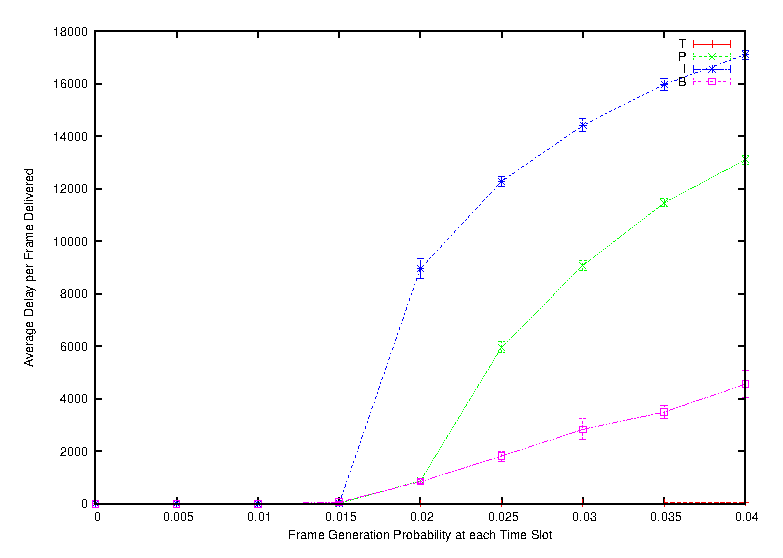
\includegraphics[width=8cm]{plots/delay_big.eps}
    \caption{ }
    \label{fig:delay_big}
\end{figure}

\begin{figure}
    \centering
    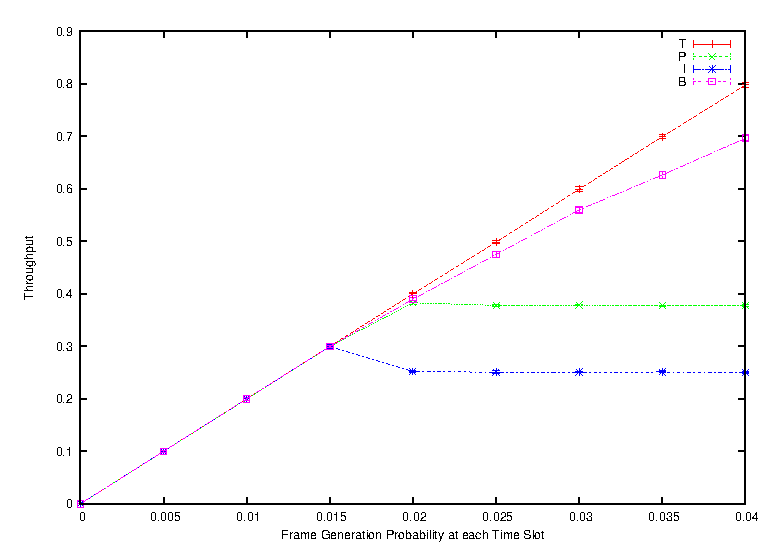
\includegraphics[width=8cm]{plots/throughput_big.eps}
    \caption{ }
    \label{fig:throughput_big}
\end{figure}

\begin{figure}
    \centering
    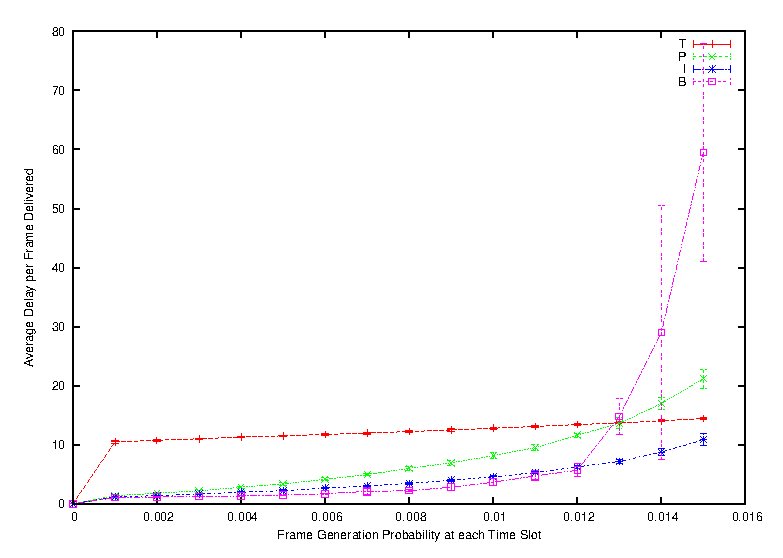
\includegraphics[width=8cm]{plots/small_delay.eps}
    \caption{ }
    \label{fig:delay_small}
\end{figure}

\begin{figure}
    \centering
    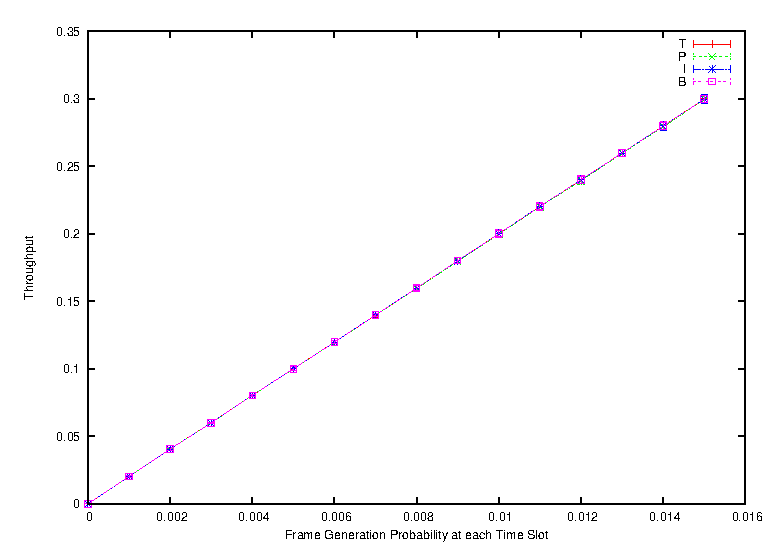
\includegraphics[width=8cm]{plots/small_throughput.eps}
    \caption{ }
    \label{fig:throughput_small}
\end{figure}

\begin{figure}
    \centering
    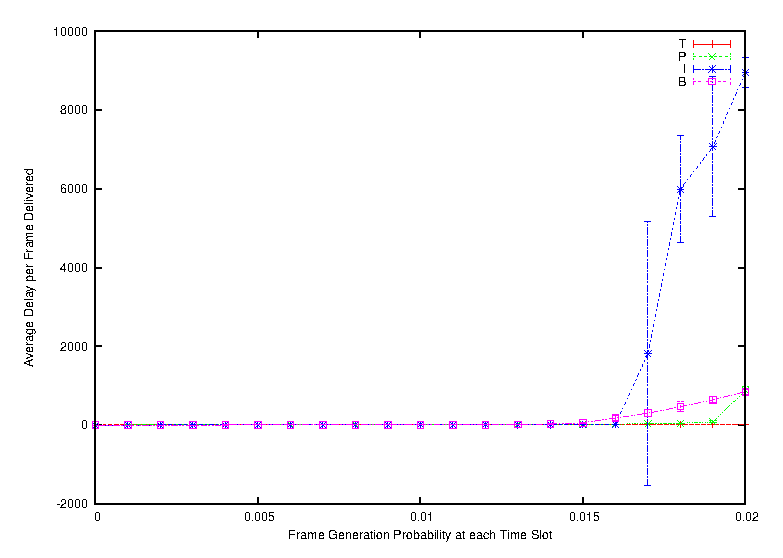
\includegraphics[width=8cm]{plots/ib_diverge_delay.eps}
    \caption{ }
    \label{fig:delay_ib}
\end{figure}

\begin{figure}
    \centering
    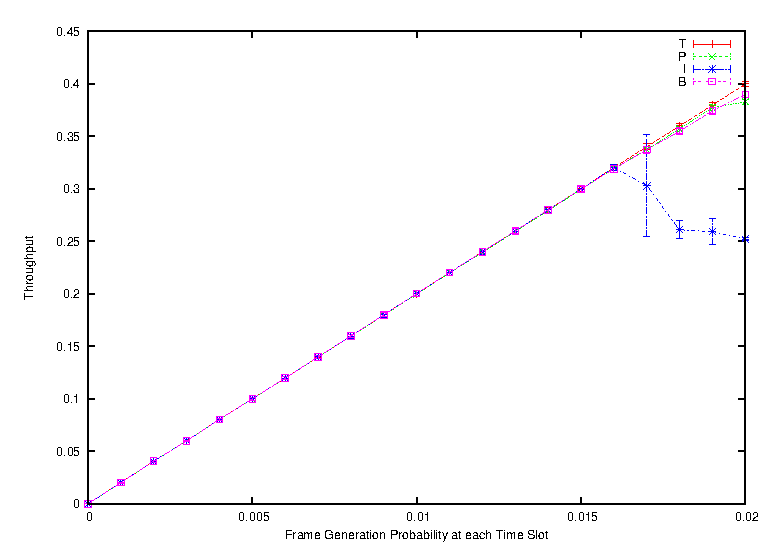
\includegraphics[width=8cm]{plots/ib_diverge_throughput.eps}
    \caption{ }
    \label{fig:throughput_ib}
\end{figure}

\begin{figure}
    \centering
    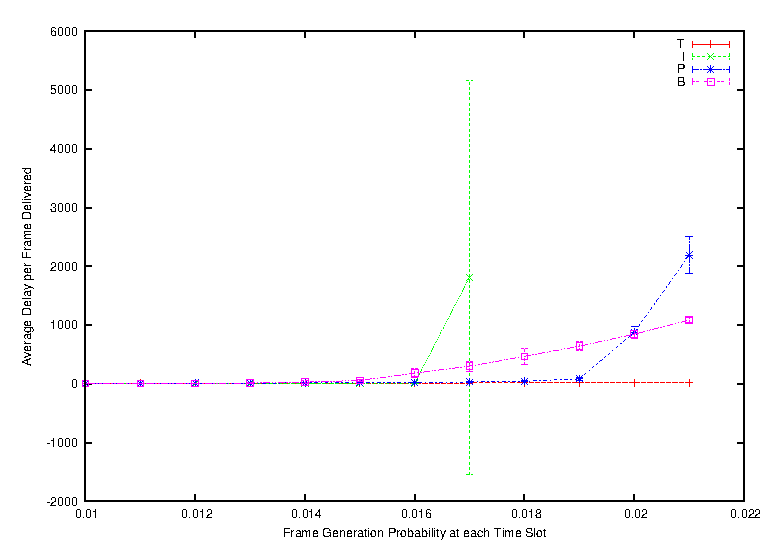
\includegraphics[width=8cm]{plots/tpbi_delay.eps}
    \caption{ }
    \label{fig:delay_diverging}
\end{figure}

\begin{figure}
    \centering
    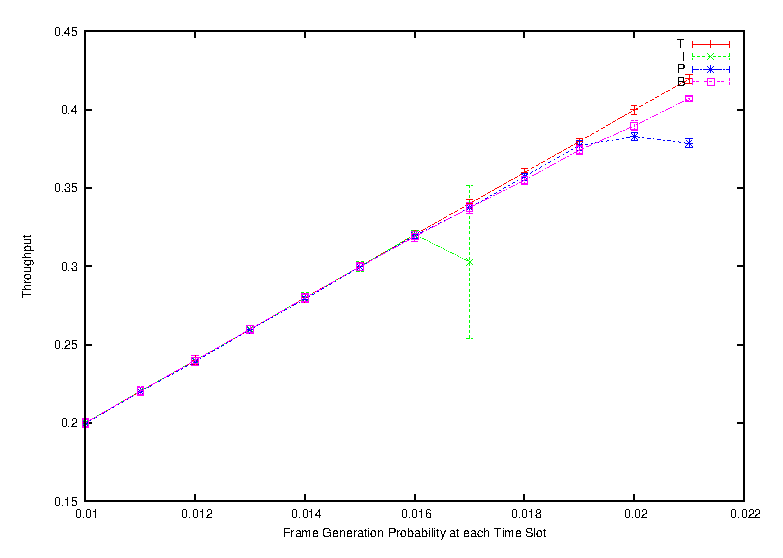
\includegraphics[width=8cm]{plots/tpbi_throughput.eps}
    \caption{ }
    \label{fig:throughput_diverging}
\end{figure}

%    In Figure~\ref{fig:kthroughput}, a plot was obtained that shows the relationship between 
%    throughput and bit error rate for different numbers of error correction blocks. $K=0$ 
%    corresponds to a transmission scheme with only error detection and no error correction.
%    For very low bit error rates, $K=0$ provides the highest simulated throughput. As bit 
%    error rate increases, the best throughput is overtaken by error correction schemes 
%    corresponding to progressively higher numbers of $K$. The highest possible value for 
%    $K$ with a frame size of 8000 bits, $K=4000$, is shown to be able to withstand the highest
%    bit error rate before collapsing to 0, but with the drawback of a drastically reduced upper
%    bound of below 50\% throughput at lower bit error rates. The relationship between
%    throughput and bit error rate for a constant $K$ appears to resemble a hyperbolic tangent.
%
%    Looking at Figure~\ref{fig:kframes}, the bit rates at which each correction scheme 
%    collapses is very visible. $K=0$ collapses in the middle range of $(0.0001, 0.001)$, and
%    $K=4000$ collapses at around 0.01.
%
%    To observe how changes to the feedback time effect the relative performance of different
%    $K$-values, in Figure~\ref{fig:a} throughput versus bit error rate was plotted for a 
%    small range of $K$ for 3 different values of $A$, where $A$ is the feedback time in bit
%    time units (Figure~\ref{fig:a10000}). Increasing A causes strong, even reductions in the 
%    throughput for all $K$-values, as well as affecting the relative performance of different 
%    $K$-values at certain ranges of bit error rate $e$. For $A=100$, $K=0$ outperforms $K=1$ 
%    for $e < 10^{-7}$,
%    and $K=0$ outperforms $K=10$ for around $e < 10^{-6}$. Increasing $A$ reduces the range where
%    correctionless schemes can outperform schemes with correction, as for $A=100000$, $K=0$ 
%    outperforms $K=1$ and $K=10$ for values of $e$ below around $10^{-7}$, $10^{-8}$ 
%    respectively.
%
%\begin{figure}
%    \centering
%    \includegraphics[width=8cm]{plots/fig1.eps}
%    \caption{ Simulated throughputs for varying bit error rates and numbers of correction
%    blocks. Error bars denote 95\% confidence intervals. Fixed parameters used were 
%    $A = 100$, $R = 10^6$, $T=5$. X-axis is log scale. }
%    \label{fig:kthroughput}
%\end{figure}
%
%\begin{figure}
%    \centering
%    \includegraphics[width=8cm]{plots/fig2.eps}
%    \caption{ Simulated average frames transmitted for each correct frame received, for
%    various bit error rates and numbers of correction blocks. Error bars denote 
%    95\% confidence intervals. Fixed parameters used were 
%    $A = 100$, $R = 10^6$, $T=5$. }
%    \label{fig:kframes}
%\end{figure}
%
%\begin{figure}
%    \centering
%    \includegraphics[width=8cm]{plots/fig5.eps}
%    \caption{ Simulated throughput response at feedback delay $A=10000$ bit time units. 
%        All other parameters are the same as those used in Figure~\ref{fig:kthroughput}.
%    }
%    \label{fig:a10000}
%\end{figure}
%
%\begin{figure}
%    \centering
%    \includegraphics[width=8cm]{plots/fig4_100.eps}
%    \includegraphics[width=8cm]{plots/fig4_10000.eps}
%    \includegraphics[width=8cm]{plots/fig4_100000.eps}
%    \caption{ Increasing values of $A$. The top plot is for $A=100$, with $R=10^7$. The middle
%    plot is for $A=10000$, with $R=10^7$. The bottom plot is for $A=100000$, with $R=10^8$.
%    $T=5$ in all cases. X-axis is log scale. } 
%    \label{fig:a}
%\end{figure}


\section*{Discussion}

%    When looking to maximize throughput, the most appropriate value for $K$, where $K$ 
%    is the number of error correction blocks,
%    is a function of the bit error rate $e$. For sufficiently low values of $e$, $K=0$ 
%    performs the best because the error rate is not high enough for the 
%    performance boosts error correction to overcome the extra overhead of sending along 
%    correction bits.
%
%    As the bit error rate increases, $K=0$ begins to suffer, as any time a single bit 
%    error is encountered, the entire frame must be retransmitted. For $K$-values greater
%    than 0, frames can withstand up to $K$ single bit errors before requiring retransmission. 
%    However, these cannot be any $K$ random bit errors in the frame, otherwise for 
%    $K=4000$ should be able to withstand $e$ up to 0.5. For $K$ single bit errors to be 
%    corrected, the $K$ errors must be distributed such that each error is in a separate 
%    correction block, which is a lower probability event than a more random scattering such that
%    a correction block contains more than one bit error, where the frame must be dropped and
%    retransmitted.
%
%    Increasing the number of correction blocks arbitrarily to maximize resilience against 
%    error is not the best approach. Using the maximum number of correction blocks possible
%    may maintain throughput without collapsing for the highest bit error rates, but for 
%    any bit error rate less than that, a slightly smaller number of correction blocks will 
%    likely give a significantly higher throughput due to the hyperbolic tangent shape of the
%    throughput curve. Also with the maximum number of correction blocks, even with an error
%    probability of zero, the throughput will be capped at 50\% since have the bits in the 
%    frame are overhead for error correction.
%
%    Higher feedback delay values were also investigated. It could be expected that the cost
%    of retransmitting a frame grows higher as feedback delays increase, and thus would
%    lend to the idea that with higher feedback delays, the relative performance of 
%    schemes utilizing receiver-size error correction would improve with respect to uncorrected
%    schemes. This was observed to be the case to some extend as seen in Figure~\ref{fig:a}, 
%    where $K=0$ remains the top performer for higher error rates at lower delays than at higher
%    delays. This effect would likely be more pronounced if the transmission scheme were a 
%    fully pipelined, sliding window scheme rather than a stop and wait scheme. Since this 
%    scheme is stop and wait, when the delay is much longer than the transmission time, 
%    throughput is decreased dramatically as the sender must wait for receiver to acknowledge
%    the sender's frames. With a fully pipelined scheme, the connection could be utilized with
%    near 100\% throughput if the error correction is able to keep up, while a correctionless
%    scheme could collapse at the same error rate with no error tolerance and such large feedback
%    delays.
%
%    In general, the simulated results from these experiments likely overestimate the throughput
%    generated by the correction schemes, as real world bit errors often come in bursts rather
%    than uniformly distributed. This would result in a higher likelihood of correction blocks
%    that contain multiple bit errors, and thus an increased rate of dropped frames that 
%    must be retransmitted.

\section*{Conclusions}

%    We have observed that a transmission scheme that splits frames into multiple Hamming's 
%    Single Bit Correction blocks can increase the scheme's resilience to higher bit rate 
%    errors with an effect proportional to the number of correction blocks per frame used. 
%    However, the correction comes at a price as throughput at lower than critical bit error
%    rates is proportionally reduced with more correction blocks. Increasing the number of 
%    correction blocks can increase the critical bit error rate where throughput collapses 
%    to zero by 
%    over an order of magnitude without sacrificing more than a 50\% decrease in throughput
%    at non-critical error levels. For situations with higher feedback delays, the improvements
%    offered by increased correction are
%    increased slightly, but for fully pipelined transmission schemes the effect is expected 
%    to be larger.

\end{document}
